\documentclass[1p]{elsarticle_modified}
%\bibliographystyle{elsarticle-num}

%\usepackage[colorlinks]{hyperref}
%\usepackage{abbrmath_seonhwa} %\Abb, \Ascr, \Acal ,\Abf, \Afrak
\usepackage{amsfonts}
\usepackage{amssymb}
\usepackage{amsmath}
\usepackage{amsthm}
\usepackage{scalefnt}
\usepackage{amsbsy}
\usepackage{kotex}
\usepackage{caption}
\usepackage{subfig}
\usepackage{color}
\usepackage{graphicx}
\usepackage{xcolor} %% white, black, red, green, blue, cyan, magenta, yellow
\usepackage{float}
\usepackage{setspace}
\usepackage{hyperref}

\usepackage{tikz}
\usetikzlibrary{arrows}

\usepackage{multirow}
\usepackage{array} % fixed length table
\usepackage{hhline}

%%%%%%%%%%%%%%%%%%%%%
\makeatletter
\renewcommand*\env@matrix[1][\arraystretch]{%
	\edef\arraystretch{#1}%
	\hskip -\arraycolsep
	\let\@ifnextchar\new@ifnextchar
	\array{*\c@MaxMatrixCols c}}
\makeatother %https://tex.stackexchange.com/questions/14071/how-can-i-increase-the-line-spacing-in-a-matrix
%%%%%%%%%%%%%%%

\usepackage[normalem]{ulem}

\newcommand{\msout}[1]{\ifmmode\text{\sout{\ensuremath{#1}}}\else\sout{#1}\fi}
%SOURCE: \msout is \stkout macro in https://tex.stackexchange.com/questions/20609/strikeout-in-math-mode

\newcommand{\cancel}[1]{
	\ifmmode
	{\color{red}\msout{#1}}
	\else
	{\color{red}\sout{#1}}
	\fi
}

\newcommand{\add}[1]{
	{\color{blue}\uwave{#1}}
}

\newcommand{\replace}[2]{
	\ifmmode
	{\color{red}\msout{#1}}{\color{blue}\uwave{#2}}
	\else
	{\color{red}\sout{#1}}{\color{blue}\uwave{#2}}
	\fi
}

\newcommand{\Sol}{\mathcal{S}} %segment
\newcommand{\D}{D} %diagram
\newcommand{\A}{\mathcal{A}} %arc


%%%%%%%%%%%%%%%%%%%%%%%%%%%%%5 test

\def\sl{\operatorname{\textup{SL}}(2,\Cbb)}
\def\psl{\operatorname{\textup{PSL}}(2,\Cbb)}
\def\quan{\mkern 1mu \triangleright \mkern 1mu}

\theoremstyle{definition}
\newtheorem{thm}{Theorem}[section]
\newtheorem{prop}[thm]{Proposition}
\newtheorem{lem}[thm]{Lemma}
\newtheorem{ques}[thm]{Question}
\newtheorem{cor}[thm]{Corollary}
\newtheorem{defn}[thm]{Definition}
\newtheorem{exam}[thm]{Example}
\newtheorem{rmk}[thm]{Remark}
\newtheorem{alg}[thm]{Algorithm}

\newcommand{\I}{\sqrt{-1}}
\begin{document}

%\begin{frontmatter}
%
%\title{Boundary parabolic representations of knots up to 8 crossings}
%
%%% Group authors per affiliation:
%\author{Yunhi Cho} 
%\address{Department of Mathematics, University of Seoul, Seoul, Korea}
%\ead{yhcho@uos.ac.kr}
%
%
%\author{Seonhwa Kim} %\fnref{s_kim}}
%\address{Center for Geometry and Physics, Institute for Basic Science, Pohang, 37673, Korea}
%\ead{ryeona17@ibs.re.kr}
%
%\author{Hyuk Kim}
%\address{Department of Mathematical Sciences, Seoul National University, Seoul 08826, Korea}
%\ead{hyukkim@snu.ac.kr}
%
%\author{Seokbeom Yoon}
%\address{Department of Mathematical Sciences, Seoul National University, Seoul, 08826,  Korea}
%\ead{sbyoon15@snu.ac.kr}
%
%\begin{abstract}
%We find all boundary parabolic representation of knots up to 8 crossings.
%
%\end{abstract}
%\begin{keyword}
%    \MSC[2010] 57M25 
%\end{keyword}
%
%\end{frontmatter}

%\linenumbers
%\tableofcontents
%
\newcommand\colored[1]{\textcolor{white}{\rule[-0.35ex]{0.8em}{1.4ex}}\kern-0.8em\color{red} #1}%
%\newcommand\colored[1]{\textcolor{white}{ #1}\kern-2.17ex	\textcolor{white}{ #1}\kern-1.81ex	\textcolor{white}{ #1}\kern-2.15ex\color{red}#1	}

{\Large $\underline{10_{149}~(K10n_{11})}$}

\setlength{\tabcolsep}{10pt}
\renewcommand{\arraystretch}{1.6}
\vspace{1cm}\begin{tabular}{m{100pt}>{\centering\arraybackslash}m{274pt}}
\multirow{5}{120pt}{
	\centering
	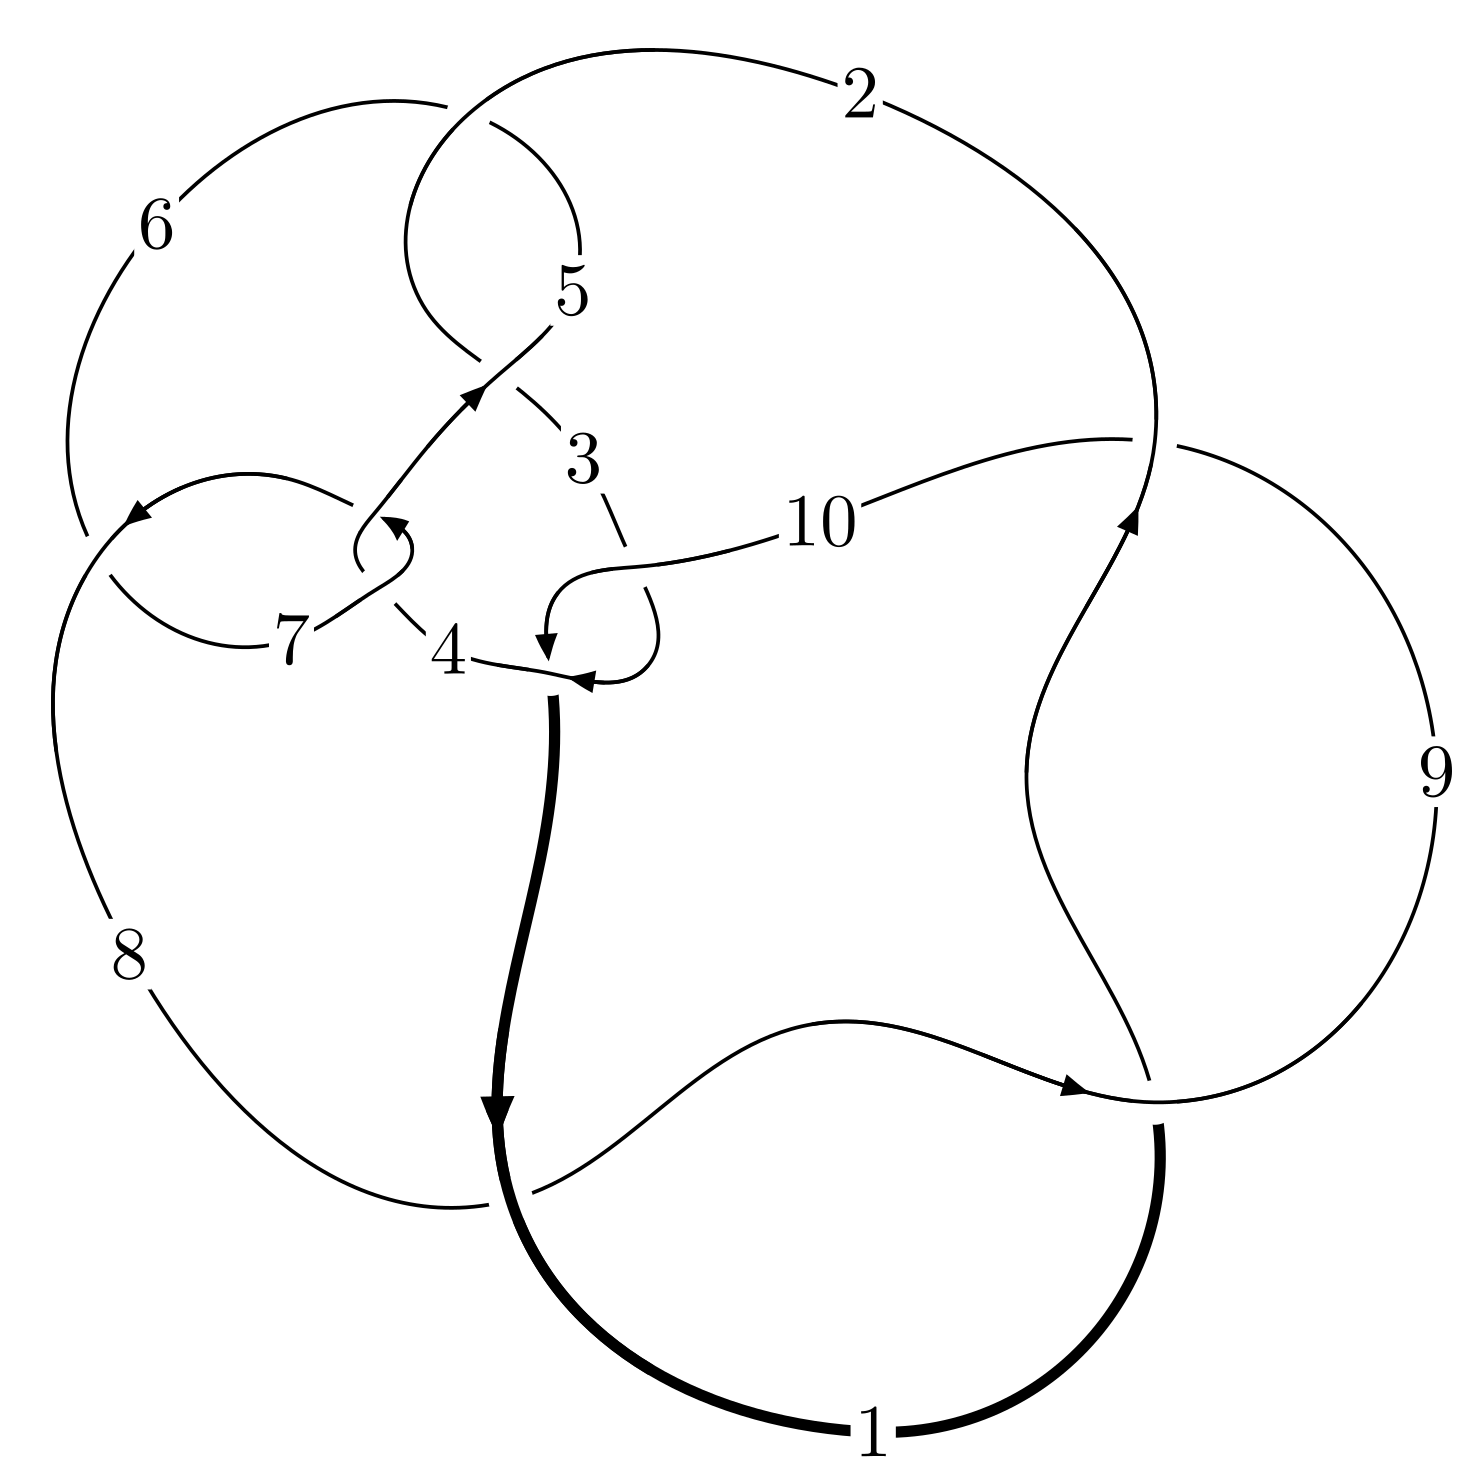
\includegraphics[width=112pt]{../../../GIT/diagram.site/Diagrams/png/233_10_149.png}\\
\ \ \ A knot diagram\footnotemark}&
\allowdisplaybreaks
\textbf{Linearized knot diagam} \\
\cline{2-2}
 &
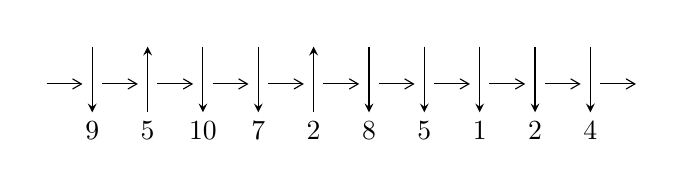
\begin{tikzpicture}[x=20pt, y=17pt]
	% nodes
	\node (C0) at (0, 0) {};
	\node (C1) at (1, 0) {};
	\node (C1U) at (1, +1) {};
	\node (C1D) at (1, -1) {9};

	\node (C2) at (2, 0) {};
	\node (C2U) at (2, +1) {};
	\node (C2D) at (2, -1) {5};

	\node (C3) at (3, 0) {};
	\node (C3U) at (3, +1) {};
	\node (C3D) at (3, -1) {10};

	\node (C4) at (4, 0) {};
	\node (C4U) at (4, +1) {};
	\node (C4D) at (4, -1) {7};

	\node (C5) at (5, 0) {};
	\node (C5U) at (5, +1) {};
	\node (C5D) at (5, -1) {2};

	\node (C6) at (6, 0) {};
	\node (C6U) at (6, +1) {};
	\node (C6D) at (6, -1) {8};

	\node (C7) at (7, 0) {};
	\node (C7U) at (7, +1) {};
	\node (C7D) at (7, -1) {5};

	\node (C8) at (8, 0) {};
	\node (C8U) at (8, +1) {};
	\node (C8D) at (8, -1) {1};

	\node (C9) at (9, 0) {};
	\node (C9U) at (9, +1) {};
	\node (C9D) at (9, -1) {2};

	\node (C10) at (10, 0) {};
	\node (C10U) at (10, +1) {};
	\node (C10D) at (10, -1) {4};
	\node (C11) at (11, 0) {};

	% arrows
	\draw[->,>={angle 60}]
	(C0) edge (C1) (C1) edge (C2) (C2) edge (C3) (C3) edge (C4) (C4) edge (C5) (C5) edge (C6) (C6) edge (C7) (C7) edge (C8) (C8) edge (C9) (C9) edge (C10) (C10) edge (C11) ;	\draw[->,>=stealth]
	(C1U) edge (C1D) (C2D) edge (C2U) (C3U) edge (C3D) (C4U) edge (C4D) (C5D) edge (C5U) (C6U) edge (C6D) (C7U) edge (C7D) (C8U) edge (C8D) (C9U) edge (C9D) (C10U) edge (C10D) ;
	\end{tikzpicture} \\
\hhline{~~} \\& 
\textbf{Solving Sequence} \\ \cline{2-2} 
 &
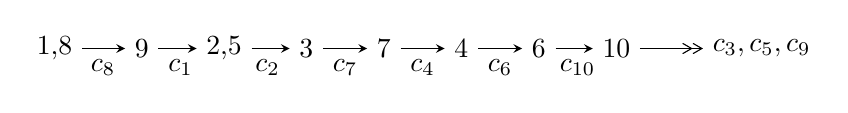
\begin{tikzpicture}[x=28pt, y=7pt]
	% node
	\node (A0) at (-1/8, 0) {1,8};
	\node (A1) at (1, 0) {9};
	\node (A2) at (33/16, 0) {2,5};
	\node (A3) at (25/8, 0) {3};
	\node (A4) at (33/8, 0) {7};
	\node (A5) at (41/8, 0) {4};
	\node (A6) at (49/8, 0) {6};
	\node (A7) at (57/8, 0) {10};
	\node (C1) at (1/2, -1) {$c_{8}$};
	\node (C2) at (3/2, -1) {$c_{1}$};
	\node (C3) at (21/8, -1) {$c_{2}$};
	\node (C4) at (29/8, -1) {$c_{7}$};
	\node (C5) at (37/8, -1) {$c_{4}$};
	\node (C6) at (45/8, -1) {$c_{6}$};
	\node (C7) at (53/8, -1) {$c_{10}$};
	\node (A8) at (9, 0) {$c_{3},c_{5},c_{9}$};

	% edge
	\draw[->,>=stealth]	
	(A0) edge (A1) (A1) edge (A2) (A2) edge (A3) (A3) edge (A4) (A4) edge (A5) (A5) edge (A6) (A6) edge (A7) ;
	\draw[->>,>={angle 60}]	
	(A7) edge (A8);
\end{tikzpicture} \\ 

\end{tabular} \\

\footnotetext{
The image of knot diagram is generated by the software ``\textbf{Draw programme}" developed by Andrew Bartholomew(\url{http://www.layer8.co.uk/maths/draw/index.htm\#Running-draw}), where we modified some parts for our purpose(\url{https://github.com/CATsTAILs/LinksPainter}).
}\phantom \\ \newline 
\centering \textbf{Ideals for irreducible components\footnotemark of $X_{\text{par}}$} 
 
\begin{align*}
I^u_{1}&=\langle 
-876201 u^{21}-2322990 u^{20}+\cdots+4026049 b+4761515,\\
\phantom{I^u_{1}}&\phantom{= \langle  }2437160 u^{21}+3033235 u^{20}+\cdots+4026049 a-11137406,\;u^{22}+2 u^{21}+\cdots-5 u+1\rangle \\
I^u_{2}&=\langle 
b+1,\;a- u-1,\;u^2+u-1\rangle \\
\\
\end{align*}
\raggedright * 2 irreducible components of $\dim_{\mathbb{C}}=0$, with total 24 representations.\\
\footnotetext{All coefficients of polynomials are rational numbers. But the coefficients are sometimes approximated in decimal forms when there is not enough margin.}
\newpage
\renewcommand{\arraystretch}{1}
\centering \section*{I. $I^u_{1}= \langle -8.76\times10^{5} u^{21}-2.32\times10^{6} u^{20}+\cdots+4.03\times10^{6} b+4.76\times10^{6},\;2.44\times10^{6} u^{21}+3.03\times10^{6} u^{20}+\cdots+4.03\times10^{6} a-1.11\times10^{7},\;u^{22}+2 u^{21}+\cdots-5 u+1 \rangle$}
\flushleft \textbf{(i) Arc colorings}\\
\begin{tabular}{m{7pt} m{180pt} m{7pt} m{180pt} }
\flushright $a_{1}=$&$\begin{pmatrix}0\\u\end{pmatrix}$ \\
\flushright $a_{8}=$&$\begin{pmatrix}1\\0\end{pmatrix}$ \\
\flushright $a_{9}=$&$\begin{pmatrix}1\\u^2\end{pmatrix}$ \\
\flushright $a_{2}=$&$\begin{pmatrix}- u\\- u^3+u\end{pmatrix}$ \\
\flushright $a_{5}=$&$\begin{pmatrix}-0.605348 u^{21}-0.753402 u^{20}+\cdots+2.33325 u+2.76634\\0.217633 u^{21}+0.576990 u^{20}+\cdots+0.524775 u-1.18268\end{pmatrix}$ \\
\flushright $a_{3}=$&$\begin{pmatrix}-0.411423 u^{21}-1.40224 u^{20}+\cdots-0.181636 u+1.11034\\-0.245107 u^{21}+0.325510 u^{20}+\cdots+2.34715 u-0.644858\end{pmatrix}$ \\
\flushright $a_{7}=$&$\begin{pmatrix}-0.796242 u^{21}-1.56338 u^{20}+\cdots+1.14222 u+4.11733\\0.129468 u^{21}+0.692040 u^{20}+\cdots+0.900899 u-1.26929\end{pmatrix}$ \\
\flushright $a_{4}=$&$\begin{pmatrix}0.400579 u^{21}+1.80305 u^{20}+\cdots+4.09317 u-2.11533\\0.823670 u^{21}+0.230100 u^{20}+\cdots-4.24775 u+0.826769\end{pmatrix}$ \\
\flushright $a_{6}=$&$\begin{pmatrix}-0.666774 u^{21}-0.871340 u^{20}+\cdots+2.04312 u+2.84804\\0.129468 u^{21}+0.692040 u^{20}+\cdots+0.900899 u-1.26929\end{pmatrix}$ \\
\flushright $a_{10}=$&$\begin{pmatrix}- u^2+1\\- u^4+2 u^2\end{pmatrix}$\\&\end{tabular}
\flushleft \textbf{(ii) Obstruction class $= -1$}\\~\\
\flushleft \textbf{(iii) Cusp Shapes $= -\frac{18273594}{4026049} u^{21}-\frac{33446853}{4026049} u^{20}+\cdots+\frac{47627074}{4026049} u-\frac{9739867}{4026049}$}\\~\\
\newpage\renewcommand{\arraystretch}{1}
\flushleft \textbf{(iv) u-Polynomials at the component}\newline \\
\begin{tabular}{m{50pt}|m{274pt}}
Crossings & \hspace{64pt}u-Polynomials at each crossing \\
\hline $$\begin{aligned}c_{1},c_{8},c_{9}\end{aligned}$$&$\begin{aligned}
&u^{22}-2 u^{21}+\cdots+5 u+1
\end{aligned}$\\
\hline $$\begin{aligned}c_{2},c_{5}\end{aligned}$$&$\begin{aligned}
&u^{22}+3 u^{21}+\cdots+28 u+4
\end{aligned}$\\
\hline $$\begin{aligned}c_{3},c_{10}\end{aligned}$$&$\begin{aligned}
&u^{22}+2 u^{21}+\cdots+u+1
\end{aligned}$\\
\hline $$\begin{aligned}c_{4},c_{7}\end{aligned}$$&$\begin{aligned}
&u^{22}-3 u^{21}+\cdots-12 u+1
\end{aligned}$\\
\hline $$\begin{aligned}c_{6}\end{aligned}$$&$\begin{aligned}
&u^{22}+9 u^{21}+\cdots+120 u+1
\end{aligned}$\\
\hline
\end{tabular}\\~\\
\newpage\renewcommand{\arraystretch}{1}
\flushleft \textbf{(v) Riley Polynomials at the component}\newline \\
\begin{tabular}{m{50pt}|m{274pt}}
Crossings & \hspace{64pt}Riley Polynomials at each crossing \\
\hline $$\begin{aligned}c_{1},c_{8},c_{9}\end{aligned}$$&$\begin{aligned}
&y^{22}-18 y^{21}+\cdots-9 y+1
\end{aligned}$\\
\hline $$\begin{aligned}c_{2},c_{5}\end{aligned}$$&$\begin{aligned}
&y^{22}-15 y^{21}+\cdots-264 y+16
\end{aligned}$\\
\hline $$\begin{aligned}c_{3},c_{10}\end{aligned}$$&$\begin{aligned}
&y^{22}-6 y^{21}+\cdots-9 y+1
\end{aligned}$\\
\hline $$\begin{aligned}c_{4},c_{7}\end{aligned}$$&$\begin{aligned}
&y^{22}-9 y^{21}+\cdots-120 y+1
\end{aligned}$\\
\hline $$\begin{aligned}c_{6}\end{aligned}$$&$\begin{aligned}
&y^{22}+11 y^{21}+\cdots-12776 y+1
\end{aligned}$\\
\hline
\end{tabular}\\~\\
\newpage\flushleft \textbf{(vi) Complex Volumes and Cusp Shapes}
$$\begin{array}{c|c|c}  
\text{Solutions to }I^u_{1}& \I (\text{vol} + \sqrt{-1}CS) & \text{Cusp shape}\\
 \hline 
\begin{aligned}
u &= \phantom{-}0.137382 + 0.980052 I \\
a &= -0.517949 - 1.178400 I \\
b &= \phantom{-}1.042580 + 0.734289 I\end{aligned}
 & \phantom{-}3.27405 - 6.32540 I & -5.56731 + 5.28995 I \\ \hline\begin{aligned}
u &= \phantom{-}0.137382 - 0.980052 I \\
a &= -0.517949 + 1.178400 I \\
b &= \phantom{-}1.042580 - 0.734289 I\end{aligned}
 & \phantom{-}3.27405 + 6.32540 I & -5.56731 - 5.28995 I \\ \hline\begin{aligned}
u &= \phantom{-}1.080880 + 0.106938 I \\
a &= -0.42141 + 2.53028 I \\
b &= -0.911911 - 0.168984 I\end{aligned}
 & -3.24923 - 0.58535 I & -11.5610 - 9.1342 I \\ \hline\begin{aligned}
u &= \phantom{-}1.080880 - 0.106938 I \\
a &= -0.42141 - 2.53028 I \\
b &= -0.911911 + 0.168984 I\end{aligned}
 & -3.24923 + 0.58535 I & -11.5610 + 9.1342 I \\ \hline\begin{aligned}
u &= -0.123407 + 0.853958 I \\
a &= \phantom{-}0.00757 + 1.42496 I \\
b &= \phantom{-}0.669484 - 0.874843 I\end{aligned}
 & \phantom{-}4.43145 - 0.35468 I & -3.17978 - 0.18562 I \\ \hline\begin{aligned}
u &= -0.123407 - 0.853958 I \\
a &= \phantom{-}0.00757 - 1.42496 I \\
b &= \phantom{-}0.669484 + 0.874843 I\end{aligned}
 & \phantom{-}4.43145 + 0.35468 I & -3.17978 + 0.18562 I \\ \hline\begin{aligned}
u &= -1.207460 + 0.170395 I \\
a &= -0.225304 - 1.032490 I \\
b &= -1.044530 + 0.860049 I\end{aligned}
 & -4.60553 + 3.49423 I & -13.3144 - 6.3296 I \\ \hline\begin{aligned}
u &= -1.207460 - 0.170395 I \\
a &= -0.225304 + 1.032490 I \\
b &= -1.044530 - 0.860049 I\end{aligned}
 & -4.60553 - 3.49423 I & -13.3144 + 6.3296 I \\ \hline\begin{aligned}
u &= -1.22419\phantom{ +0.000000I} \\
a &= -0.613520\phantom{ +0.000000I} \\
b &= -1.60485\phantom{ +0.000000I}\end{aligned}
 & -6.34803\phantom{ +0.000000I} & -16.5000\phantom{ +0.000000I} \\ \hline\begin{aligned}
u &= \phantom{-}0.736463\phantom{ +0.000000I} \\
a &= \phantom{-}0.700417\phantom{ +0.000000I} \\
b &= \phantom{-}0.0940544\phantom{ +0.000000I}\end{aligned}
 & -1.10354\phantom{ +0.000000I} & -8.74830\phantom{ +0.000000I}\\
 \hline 
 \end{array}$$\newpage$$\begin{array}{c|c|c}  
\text{Solutions to }I^u_{1}& \I (\text{vol} + \sqrt{-1}CS) & \text{Cusp shape}\\
 \hline 
\begin{aligned}
u &= -1.195650 + 0.411381 I \\
a &= -0.358621 - 0.478444 I \\
b &= \phantom{-}0.384535 + 1.127130 I\end{aligned}
 & \phantom{-}1.13790 + 4.89828 I & -6.90240 - 4.82636 I \\ \hline\begin{aligned}
u &= -1.195650 - 0.411381 I \\
a &= -0.358621 + 0.478444 I \\
b &= \phantom{-}0.384535 - 1.127130 I\end{aligned}
 & \phantom{-}1.13790 - 4.89828 I & -6.90240 + 4.82636 I \\ \hline\begin{aligned}
u &= \phantom{-}1.154470 + 0.562023 I \\
a &= -0.253567 + 0.037384 I \\
b &= \phantom{-}0.770295 - 0.637284 I\end{aligned}
 & \phantom{-}0.148418 + 0.912400 I & -7.06168 - 2.22739 I \\ \hline\begin{aligned}
u &= \phantom{-}1.154470 - 0.562023 I \\
a &= -0.253567 - 0.037384 I \\
b &= \phantom{-}0.770295 + 0.637284 I\end{aligned}
 & \phantom{-}0.148418 - 0.912400 I & -7.06168 + 2.22739 I \\ \hline\begin{aligned}
u &= \phantom{-}1.38990 + 0.37870 I \\
a &= \phantom{-}0.880502 - 0.916687 I \\
b &= \phantom{-}0.934548 + 0.639349 I\end{aligned}
 & -0.37121 - 4.08988 I & -7.66142 + 3.87499 I \\ \hline\begin{aligned}
u &= \phantom{-}1.38990 - 0.37870 I \\
a &= \phantom{-}0.880502 + 0.916687 I \\
b &= \phantom{-}0.934548 - 0.639349 I\end{aligned}
 & -0.37121 + 4.08988 I & -7.66142 - 3.87499 I \\ \hline\begin{aligned}
u &= -1.38743 + 0.45171 I \\
a &= \phantom{-}0.618352 + 1.212720 I \\
b &= \phantom{-}1.23888 - 0.71737 I\end{aligned}
 & -1.50863 + 11.44270 I & -9.41507 - 7.02258 I \\ \hline\begin{aligned}
u &= -1.38743 - 0.45171 I \\
a &= \phantom{-}0.618352 - 1.212720 I \\
b &= \phantom{-}1.23888 + 0.71737 I\end{aligned}
 & -1.50863 - 11.44270 I & -9.41507 + 7.02258 I \\ \hline\begin{aligned}
u &= \phantom{-}0.096382 + 0.403421 I \\
a &= \phantom{-}2.25348 + 0.77227 I \\
b &= -0.685093 - 0.393126 I\end{aligned}
 & -0.85664 - 1.35693 I & -6.38441 + 4.83589 I \\ \hline\begin{aligned}
u &= \phantom{-}0.096382 - 0.403421 I \\
a &= \phantom{-}2.25348 - 0.77227 I \\
b &= -0.685093 + 0.393126 I\end{aligned}
 & -0.85664 + 1.35693 I & -6.38441 - 4.83589 I\\
 \hline 
 \end{array}$$\newpage$$\begin{array}{c|c|c}  
\text{Solutions to }I^u_{1}& \I (\text{vol} + \sqrt{-1}CS) & \text{Cusp shape}\\
 \hline 
\begin{aligned}
u &= -1.66272\phantom{ +0.000000I} \\
a &= \phantom{-}0.642487\phantom{ +0.000000I} \\
b &= \phantom{-}0.825081\phantom{ +0.000000I}\end{aligned}
 & -10.1504\phantom{ +0.000000I} & \phantom{-}0.707930\phantom{ +0.000000I} \\ \hline\begin{aligned}
u &= \phantom{-}0.260308\phantom{ +0.000000I} \\
a &= \phantom{-}3.30452\phantom{ +0.000000I} \\
b &= -1.11185\phantom{ +0.000000I}\end{aligned}
 & -2.22827\phantom{ +0.000000I} & \phantom{-}0.635130\phantom{ +0.000000I}\\
 \hline 
 \end{array}$$\newpage\newpage\renewcommand{\arraystretch}{1}
\centering \section*{II. $I^u_{2}= \langle b+1,\;a- u-1,\;u^2+u-1 \rangle$}
\flushleft \textbf{(i) Arc colorings}\\
\begin{tabular}{m{7pt} m{180pt} m{7pt} m{180pt} }
\flushright $a_{1}=$&$\begin{pmatrix}0\\u\end{pmatrix}$ \\
\flushright $a_{8}=$&$\begin{pmatrix}1\\0\end{pmatrix}$ \\
\flushright $a_{9}=$&$\begin{pmatrix}1\\- u+1\end{pmatrix}$ \\
\flushright $a_{2}=$&$\begin{pmatrix}- u\\- u+1\end{pmatrix}$ \\
\flushright $a_{5}=$&$\begin{pmatrix}u+1\\-1\end{pmatrix}$ \\
\flushright $a_{3}=$&$\begin{pmatrix}- u\\- u+1\end{pmatrix}$ \\
\flushright $a_{7}=$&$\begin{pmatrix}u+2\\-1\end{pmatrix}$ \\
\flushright $a_{4}=$&$\begin{pmatrix}-1\\0\end{pmatrix}$ \\
\flushright $a_{6}=$&$\begin{pmatrix}u+1\\-1\end{pmatrix}$ \\
\flushright $a_{10}=$&$\begin{pmatrix}u\\u\end{pmatrix}$\\&\end{tabular}
\flushleft \textbf{(ii) Obstruction class $= 1$}\\~\\
\flushleft \textbf{(iii) Cusp Shapes $= -21$}\\~\\
\newpage\renewcommand{\arraystretch}{1}
\flushleft \textbf{(iv) u-Polynomials at the component}\newline \\
\begin{tabular}{m{50pt}|m{274pt}}
Crossings & \hspace{64pt}u-Polynomials at each crossing \\
\hline $$\begin{aligned}c_{1},c_{3}\end{aligned}$$&$\begin{aligned}
&u^2- u-1
\end{aligned}$\\
\hline $$\begin{aligned}c_{2},c_{5}\end{aligned}$$&$\begin{aligned}
&u^2
\end{aligned}$\\
\hline $$\begin{aligned}c_{4},c_{6}\end{aligned}$$&$\begin{aligned}
&(u-1)^2
\end{aligned}$\\
\hline $$\begin{aligned}c_{7}\end{aligned}$$&$\begin{aligned}
&(u+1)^2
\end{aligned}$\\
\hline $$\begin{aligned}c_{8},c_{9},c_{10}\end{aligned}$$&$\begin{aligned}
&u^2+u-1
\end{aligned}$\\
\hline
\end{tabular}\\~\\
\newpage\renewcommand{\arraystretch}{1}
\flushleft \textbf{(v) Riley Polynomials at the component}\newline \\
\begin{tabular}{m{50pt}|m{274pt}}
Crossings & \hspace{64pt}Riley Polynomials at each crossing \\
\hline $$\begin{aligned}c_{1},c_{3},c_{8}\\c_{9},c_{10}\end{aligned}$$&$\begin{aligned}
&y^2-3 y+1
\end{aligned}$\\
\hline $$\begin{aligned}c_{2},c_{5}\end{aligned}$$&$\begin{aligned}
&y^2
\end{aligned}$\\
\hline $$\begin{aligned}c_{4},c_{6},c_{7}\end{aligned}$$&$\begin{aligned}
&(y-1)^2
\end{aligned}$\\
\hline
\end{tabular}\\~\\
\newpage\flushleft \textbf{(vi) Complex Volumes and Cusp Shapes}
$$\begin{array}{c|c|c}  
\text{Solutions to }I^u_{2}& \I (\text{vol} + \sqrt{-1}CS) & \text{Cusp shape}\\
 \hline 
\begin{aligned}
u &= \phantom{-}0.618034\phantom{ +0.000000I} \\
a &= \phantom{-}1.61803\phantom{ +0.000000I} \\
b &= -1.00000\phantom{ +0.000000I}\end{aligned}
 & -2.63189\phantom{ +0.000000I} & -21.0000\phantom{ +0.000000I} \\ \hline\begin{aligned}
u &= -1.61803\phantom{ +0.000000I} \\
a &= -0.618034\phantom{ +0.000000I} \\
b &= -1.00000\phantom{ +0.000000I}\end{aligned}
 & -10.5276\phantom{ +0.000000I} & -21.0000\phantom{ +0.000000I}\\
 \hline 
 \end{array}$$\newpage
\newpage\renewcommand{\arraystretch}{1}
\centering \section*{ III. u-Polynomials}
\begin{tabular}{m{50pt}|m{274pt}}
Crossings & \hspace{64pt}u-Polynomials at each crossing \\
\hline $$\begin{aligned}c_{1}\end{aligned}$$&$\begin{aligned}
&(u^2- u-1)(u^{22}-2 u^{21}+\cdots+5 u+1)
\end{aligned}$\\
\hline $$\begin{aligned}c_{2},c_{5}\end{aligned}$$&$\begin{aligned}
&u^2(u^{22}+3 u^{21}+\cdots+28 u+4)
\end{aligned}$\\
\hline $$\begin{aligned}c_{3}\end{aligned}$$&$\begin{aligned}
&(u^2- u-1)(u^{22}+2 u^{21}+\cdots+u+1)
\end{aligned}$\\
\hline $$\begin{aligned}c_{4}\end{aligned}$$&$\begin{aligned}
&((u-1)^2)(u^{22}-3 u^{21}+\cdots-12 u+1)
\end{aligned}$\\
\hline $$\begin{aligned}c_{6}\end{aligned}$$&$\begin{aligned}
&((u-1)^2)(u^{22}+9 u^{21}+\cdots+120 u+1)
\end{aligned}$\\
\hline $$\begin{aligned}c_{7}\end{aligned}$$&$\begin{aligned}
&((u+1)^2)(u^{22}-3 u^{21}+\cdots-12 u+1)
\end{aligned}$\\
\hline $$\begin{aligned}c_{8},c_{9}\end{aligned}$$&$\begin{aligned}
&(u^2+u-1)(u^{22}-2 u^{21}+\cdots+5 u+1)
\end{aligned}$\\
\hline $$\begin{aligned}c_{10}\end{aligned}$$&$\begin{aligned}
&(u^2+u-1)(u^{22}+2 u^{21}+\cdots+u+1)
\end{aligned}$\\
\hline
\end{tabular}\newpage\renewcommand{\arraystretch}{1}
\centering \section*{ IV. Riley Polynomials}
\begin{tabular}{m{50pt}|m{274pt}}
Crossings & \hspace{64pt}Riley Polynomials at each crossing \\
\hline $$\begin{aligned}c_{1},c_{8},c_{9}\end{aligned}$$&$\begin{aligned}
&(y^2-3 y+1)(y^{22}-18 y^{21}+\cdots-9 y+1)
\end{aligned}$\\
\hline $$\begin{aligned}c_{2},c_{5}\end{aligned}$$&$\begin{aligned}
&y^2(y^{22}-15 y^{21}+\cdots-264 y+16)
\end{aligned}$\\
\hline $$\begin{aligned}c_{3},c_{10}\end{aligned}$$&$\begin{aligned}
&(y^2-3 y+1)(y^{22}-6 y^{21}+\cdots-9 y+1)
\end{aligned}$\\
\hline $$\begin{aligned}c_{4},c_{7}\end{aligned}$$&$\begin{aligned}
&((y-1)^2)(y^{22}-9 y^{21}+\cdots-120 y+1)
\end{aligned}$\\
\hline $$\begin{aligned}c_{6}\end{aligned}$$&$\begin{aligned}
&((y-1)^2)(y^{22}+11 y^{21}+\cdots-12776 y+1)
\end{aligned}$\\
\hline
\end{tabular}
\vskip 2pc
\end{document}